\documentclass{article}
\usepackage{amsmath}
\usepackage{graphicx}
\usepackage{hyperref}
\usepackage[margin=1in]{geometry}
\usepackage{placeins} % For \FloatBarrier

\title{Homework Number: Eight\\ \large Monetary Policy 2: Optimal Policy and the Role of Expectations}
\author{Team Two}
\date{July 12th, 2024}

\begin{document}

\maketitle

\section{The Loss Function of the Central Bank}

\subsection{Explanation of the Loss Function}
The loss function of a central bank is given by:
\[
L (y_t, \pi_t) = \lambda (y_t - \bar{y})^2 + (\pi_t - \bar{\pi})^2
\]

\begin{itemize}
    \item \(\lambda\): This is a weight parameter that determines the relative importance of output deviations compared to inflation deviations. A higher \(\lambda\) means the central bank places more importance on stabilizing output relative to inflation.
    \item \(y_t\): This represents the actual output in period \(t\).
    \item \(\bar{y}\): This is the target or potential output the central bank aims to achieve.
    \item \(\pi_t\): This is the actual inflation rate in period \(t\).
    \item \(\bar{\pi}\): This is the target inflation rate.
\end{itemize}

\textbf{Properties and Implications}:
\begin{itemize}
    \item The function penalizes deviations from the target output and target inflation. The central bank aims to minimize this loss function, indicating that it wants to keep both output and inflation as close to their respective targets as possible.
    \item The quadratic nature of the function implies that larger deviations from the targets are penalized more heavily than smaller deviations.
    \item If \(\lambda = 0\), the central bank does not care about output stabilization and focuses solely on inflation stabilization.
    \item If \(\lambda \to \infty\), the central bank does not care about inflation stabilization and focuses solely on output stabilization.
    \item According to Challe, this form of the loss function suggests that the central bank's policy decisions will be a trade-off between stabilizing inflation and output, depending on the value of \(\lambda\).
\end{itemize}

\noindent\rule{\linewidth}{0.5pt}
\newpage
\subsection{Graphs of the Loss Function}

\begin{figure}[ht!]
    \centering
    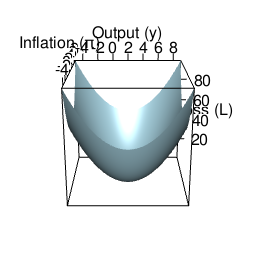
\includegraphics[width=0.8\textwidth]{/Users/cancel/Personal/Coursework/Econ425/HW8/R/central_bank_loss_function_3d_static.png}
    \caption{3D Plot of the Central Bank's Loss Function}
\label{fig:loss_function_3d}
\end{figure}

\begin{figure}[ht!]
    \centering
    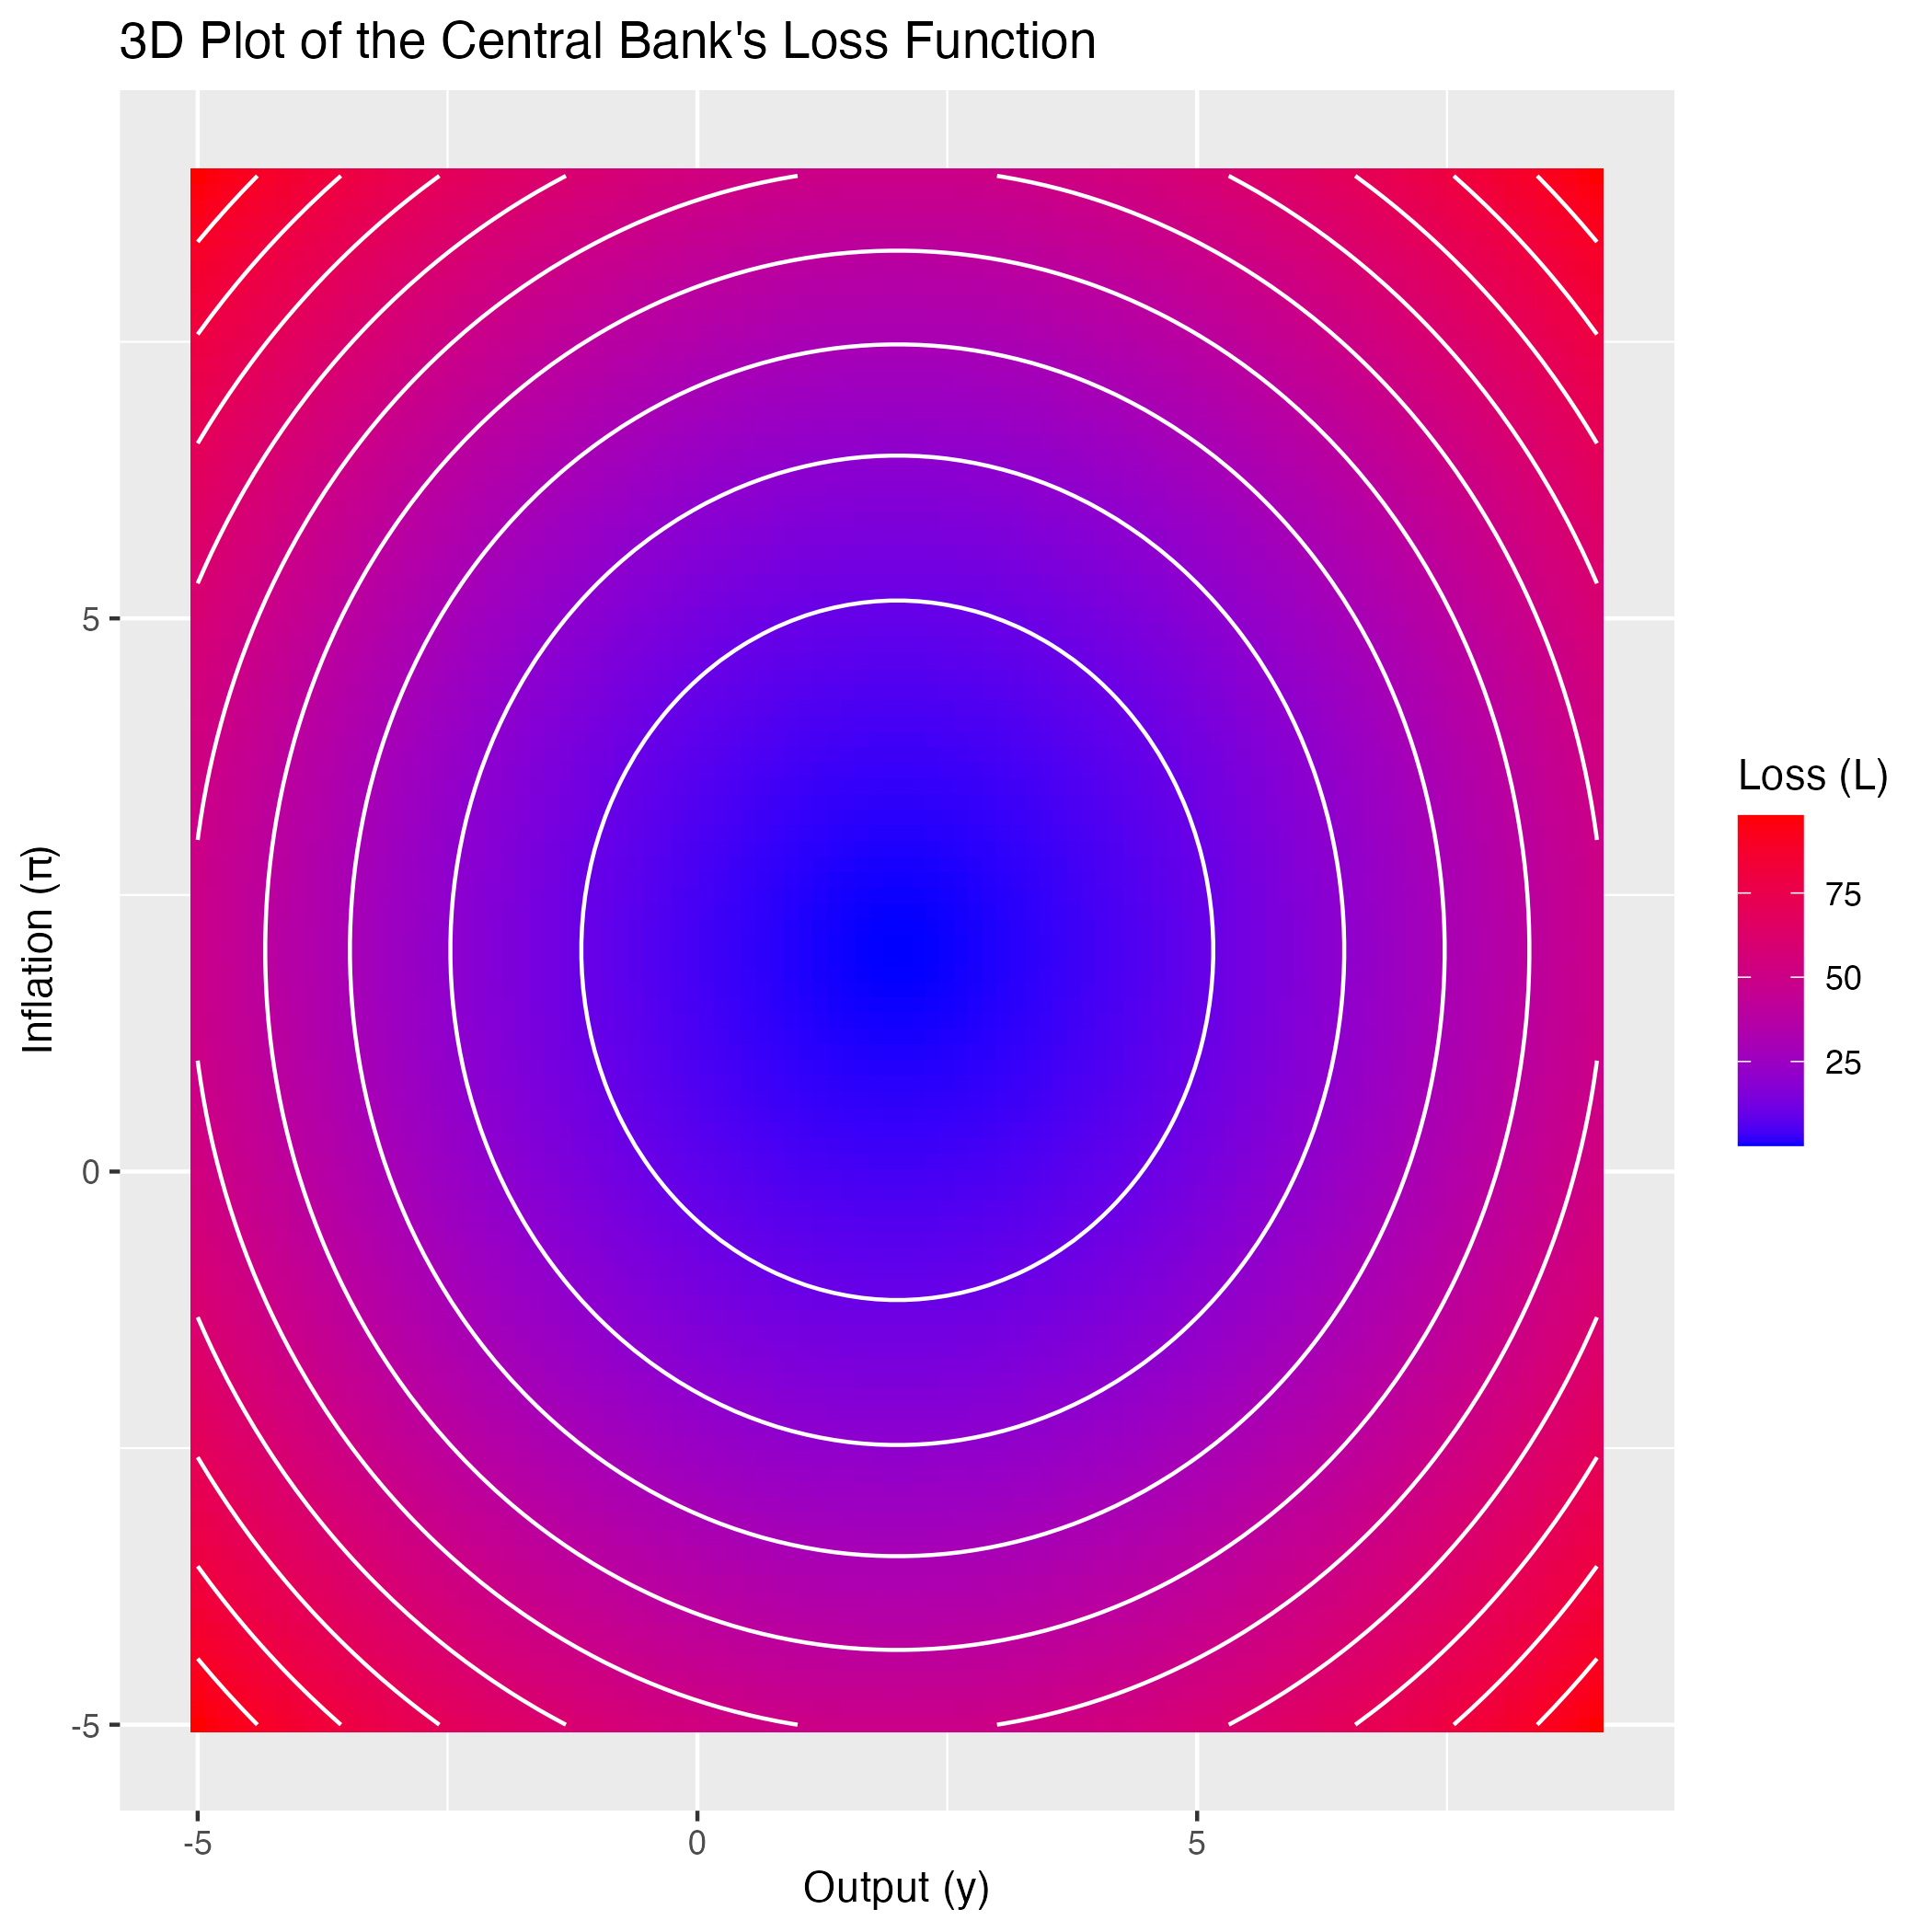
\includegraphics[width=0.8\textwidth]{/Users/cancel/Personal/Coursework/Econ425/HW8/R/central_bank_loss_function_3d_Contour.png}
    \caption{3D Contour Plot of the Central Bank's Loss Function}
\label{fig:loss_function_3d_contour}
\end{figure}

\begin{figure}[ht!]
    \centering
    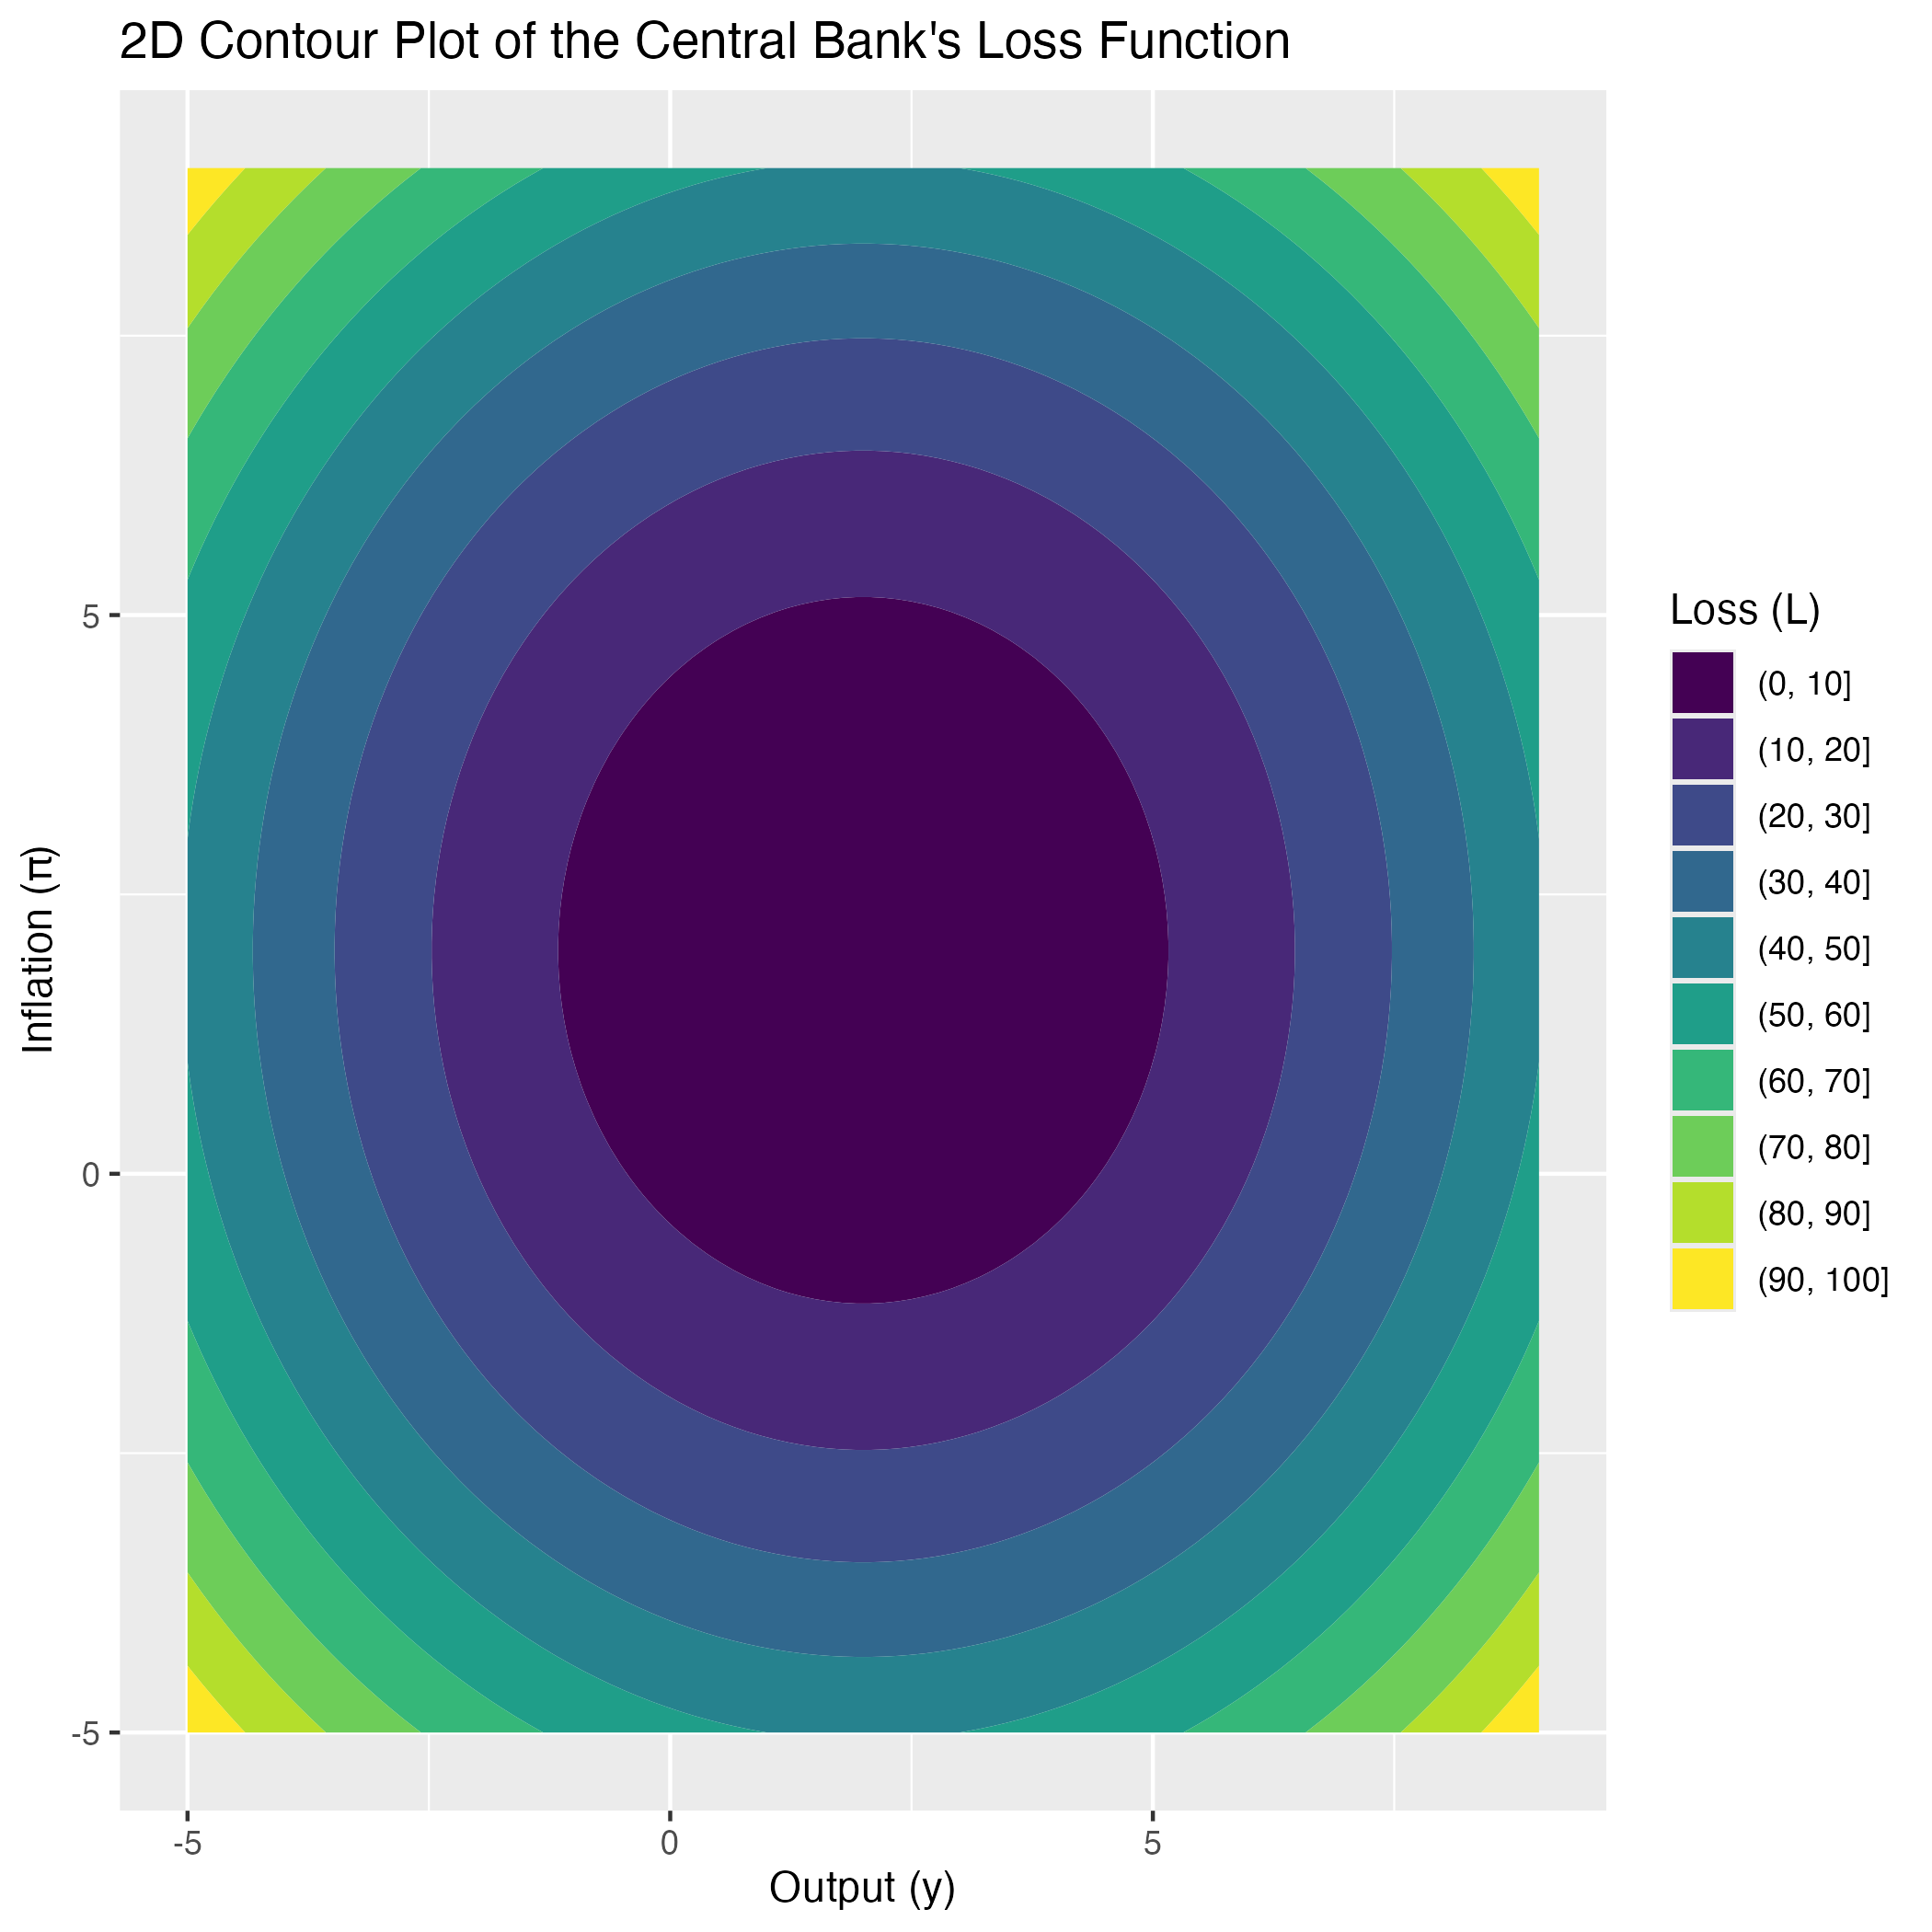
\includegraphics[width=0.8\textwidth]{/Users/cancel/Personal/Coursework/Econ425/HW8/R/central_bank_loss_function_2d.png}
    \caption{2D Contour Plot of the Central Bank's Loss Function}
\label{fig:loss_function_2d}
\end{figure}

\FloatBarrier

\subsection{Optimization Problem}

Set up the optimization problem for the intertemporal loss function:
\[
L^I_t = \sum_{k=0}^{\infty} \beta^k L (y_{t+k}, \pi_{t+k}), \quad 0 \leq \beta < 1 
\]

where the parameter \(\beta\) is the central bank's discount factor.

\textbf{Objective function:}
\[
\min \sum_{k=0}^{\infty} \beta^k \left[ \lambda (y_{t+k} - \bar{y})^2 + (\pi_{t+k} - \bar{\pi})^2 \right]
\]

\textbf{Choice variables:}
\[ y_t, \pi_t \]

\textbf{Constraints:}
\[ \text{Any constraints on } y_t \text{ and } \pi_t \text{ (e.g., Phillips curve, aggregate demand, etc.)} \]

\noindent\rule{\linewidth}{0.5pt}

\section{Optimal Monetary Policy}

\subsection{First Order Necessary Conditions (FONCs)}

To find the FONCs, we differentiate the Lagrangian with respect to \( y_t \) and \( \pi_t \) and set the derivatives to zero.

The FONCs for this problem will involve partial derivatives of the Lagrangian with respect to \( y_t \) and \( \pi_t \):
\[ \frac{\partial \mathcal{L}}{\partial y_t} = 0 \]
\[ \frac{\partial \mathcal{L}}{\partial \pi_t} = 0 \]

\subsection{Derivation of the Optimal Inflation Equation}

The optimal inflation equation can be derived from the FONCs by solving the system of equations obtained from the partial derivatives:
\[ \pi^*_t = \frac{\pi_{t-1} + \beta \pi_{t+1}}{1 + \beta + \kappa^2 / \lambda} \]

This equation represents a weighted average of past and future inflation, indicating that the central bank's optimal policy takes into account both past inflation and expected future inflation. The weights depend on the parameters \( \beta \), \( \kappa \), and \( \lambda \).

\noindent\rule{\linewidth}{0.5pt}

\subsection{Interpretation of \(\Omega\)}

Given the optimal inflation path equation:
\[ \pi^*_t = \Omega \pi^*_{t-1} \]

where:
\[ \Omega = \frac{1}{2\beta} \left[ 1 + \beta + \frac{\kappa^2}{\lambda} - \sqrt{\left(1 + \beta + \frac{\kappa^2}{\lambda}\right)^2 - 4\beta} \right] \]

\begin{itemize}
        \item \textbf{What is \(\Omega\)?} \(\Omega\) is a coefficient that determines the persistence of inflation over time. It can be considered as the rate of inflation stabilization.
        \item \textbf{What happens to \(\Omega\) when \(\beta\) increases?} When \(\beta\) increases, the weight of the future in our loss function increases, making the central bank more forward-looking. This generally decreases \(\Omega\), implying less persistence in inflation because the central bank gives more importance to stabilizing future inflation.
        \item \textbf{What happens to \(\Omega\) when \(\beta = 0\)?} When \(\beta = 0\), the central bank is myopic, focusing only on current period losses. In this case, \(\Omega = \frac{\lambda}{\lambda+\kappa^2}\) and generally holds a larger value than when \(\beta > 0\). This indicates that the central bank does not consider future inflation, and inflation persistence is maximized.
        \item \textbf{What happens to \(\Omega\) when \(\lambda\) increases?} When \(\lambda\) increases, the central bank places more weight on output stabilization relative to inflation stabilization. This typically increases \(\Omega\), indicating more inflation persistence because the central bank is more tolerant of inflation deviations.
        \item \textbf{What happens to \(\Omega\) when \(\kappa\) increases?} When \(\kappa\) increases, the sensitivity of inflation to the output gap increases. This can lead to a decrease in \(\Omega\), as the central bank becomes more responsive to changes in the output gap, reducing inflation persistence.
\end{itemize}

\noindent\rule{\linewidth}{0.5pt}

\subsection{Graphing the Optimal Inflation Path}

\begin{figure}[ht!]
    \centering
    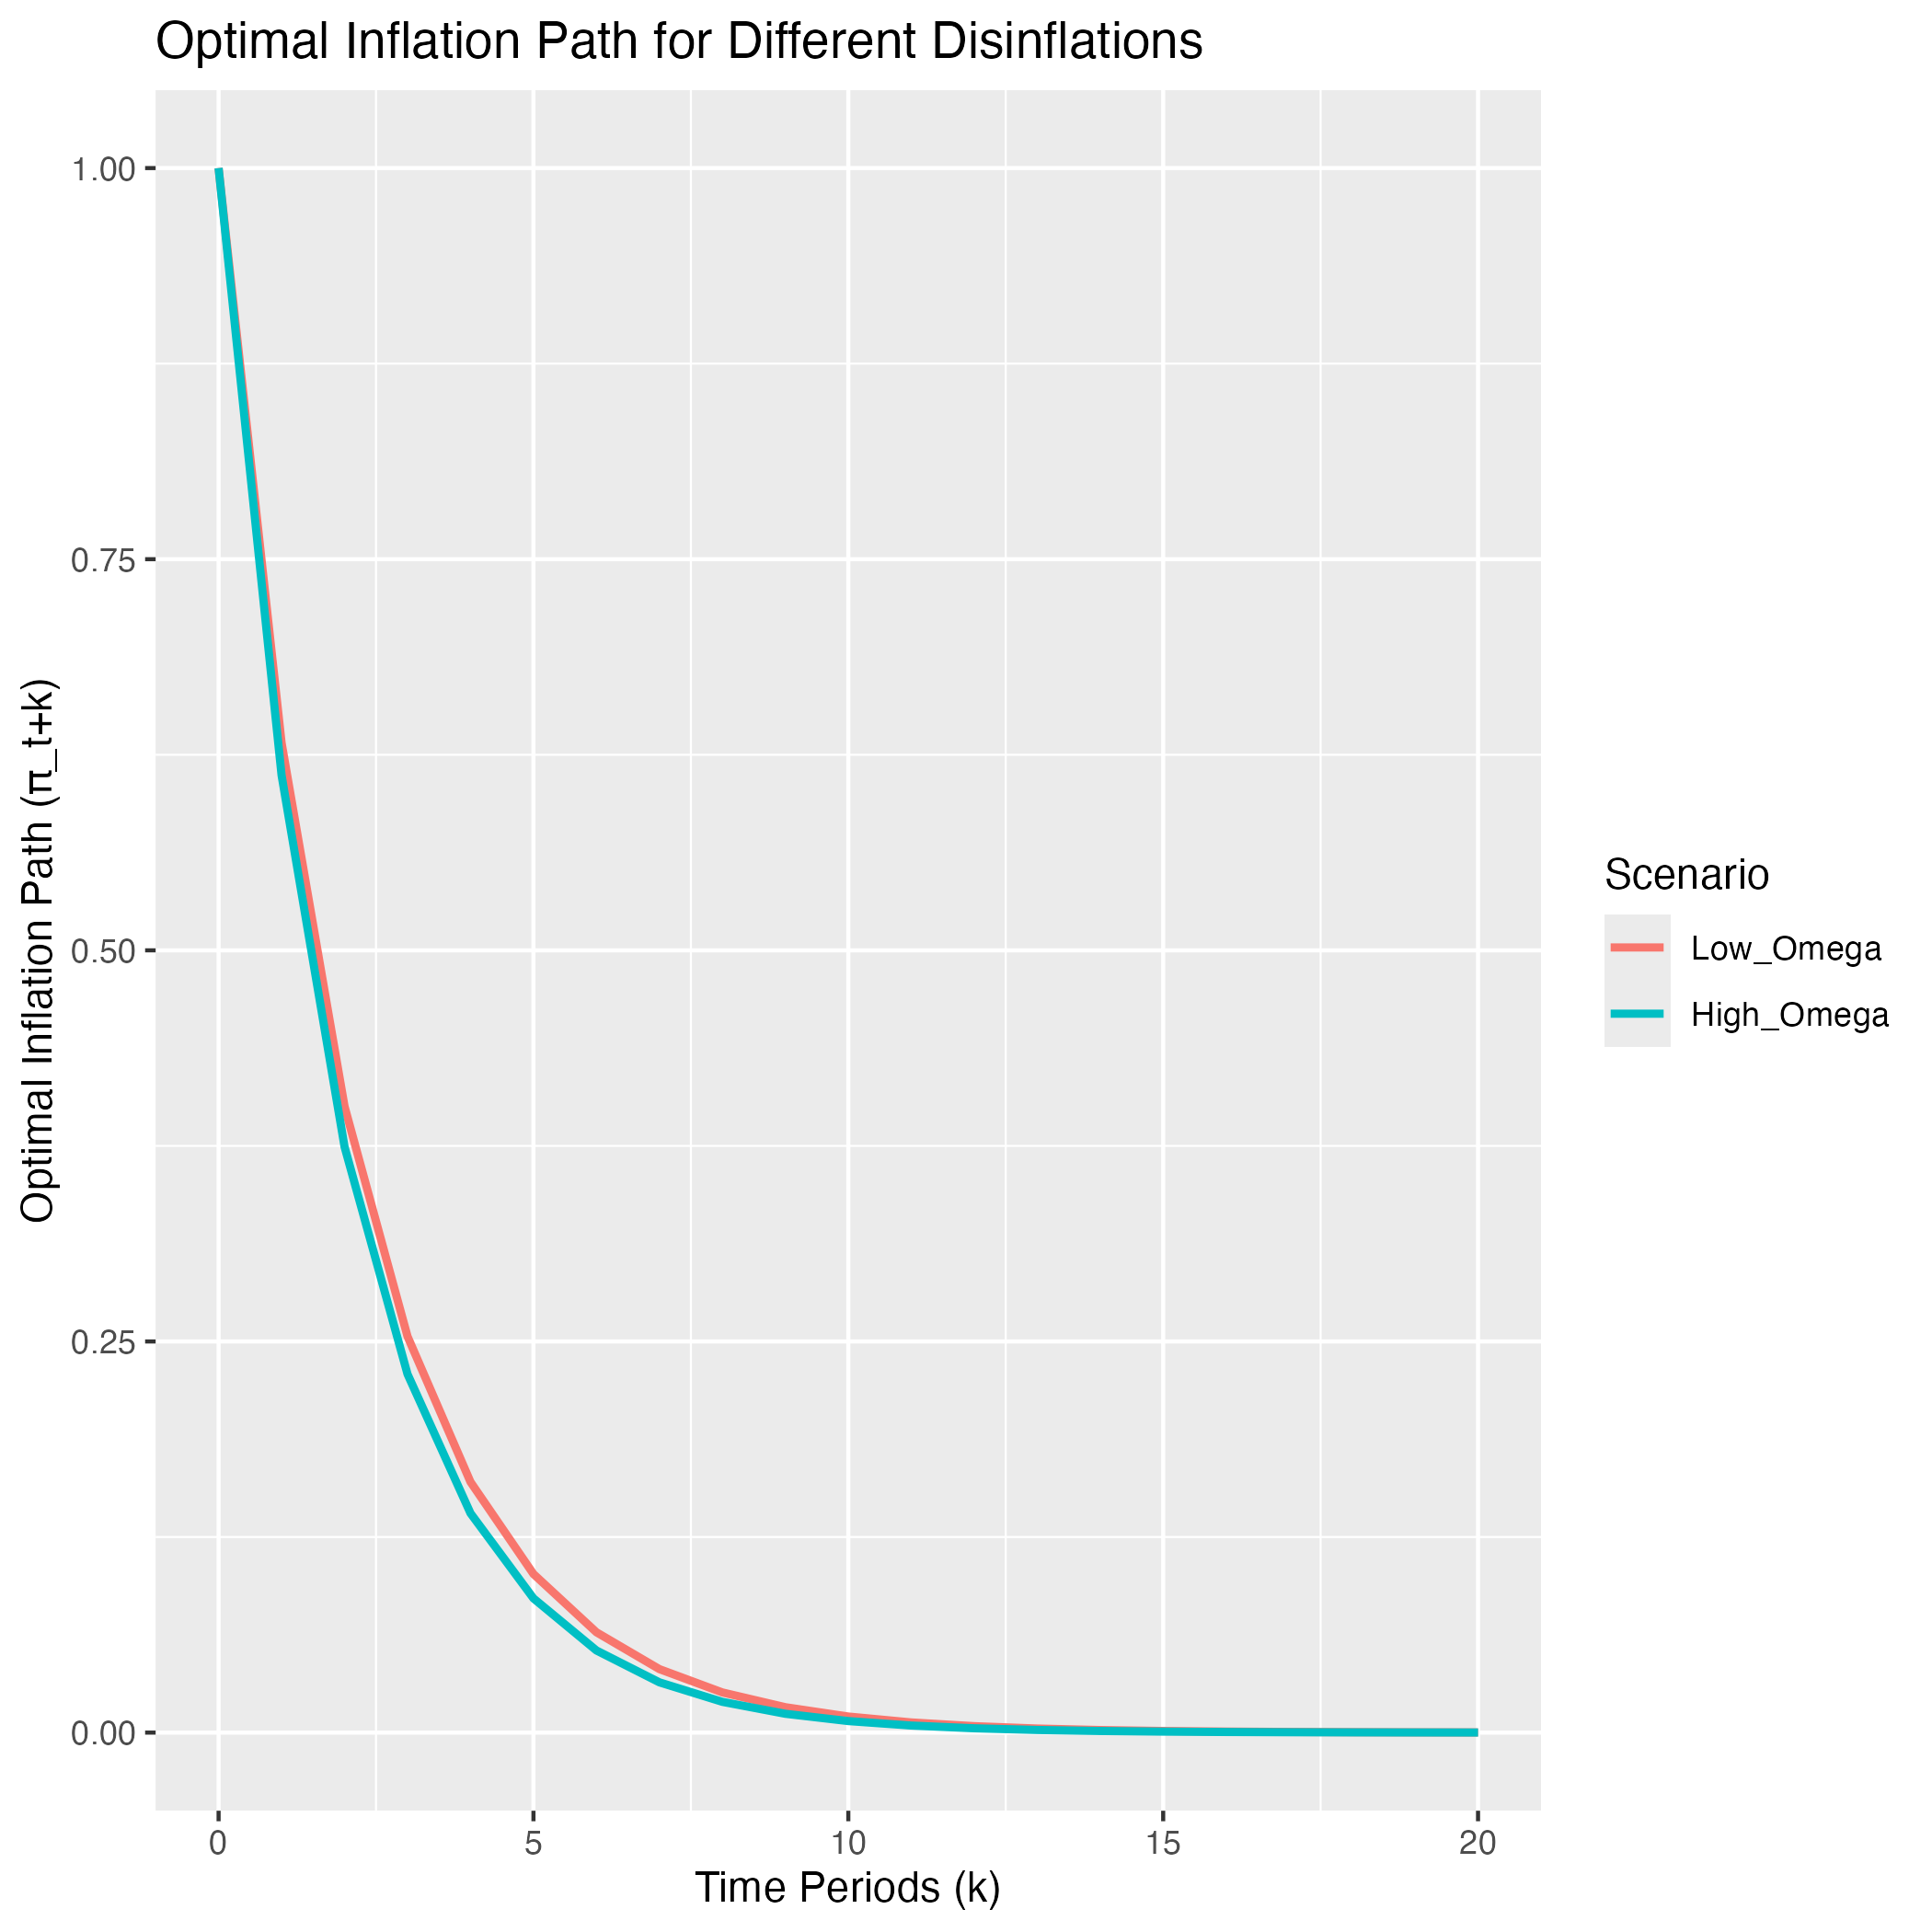
\includegraphics[width=0.8\textwidth]{/Users/cancel/Personal/Coursework/Econ425/HW8/R/optimal_inflation_path.png}
    \caption{Optimal Inflation Path for Different Disinflations}
\label{fig:optimal_inflation_path}
\end{figure}

\FloatBarrier

\noindent\rule{\linewidth}{0.5pt}

\newpage
\subsection{Graphing the Optimal Path of Output and Interest Rates}

\begin{figure}[ht!]
    \centering
    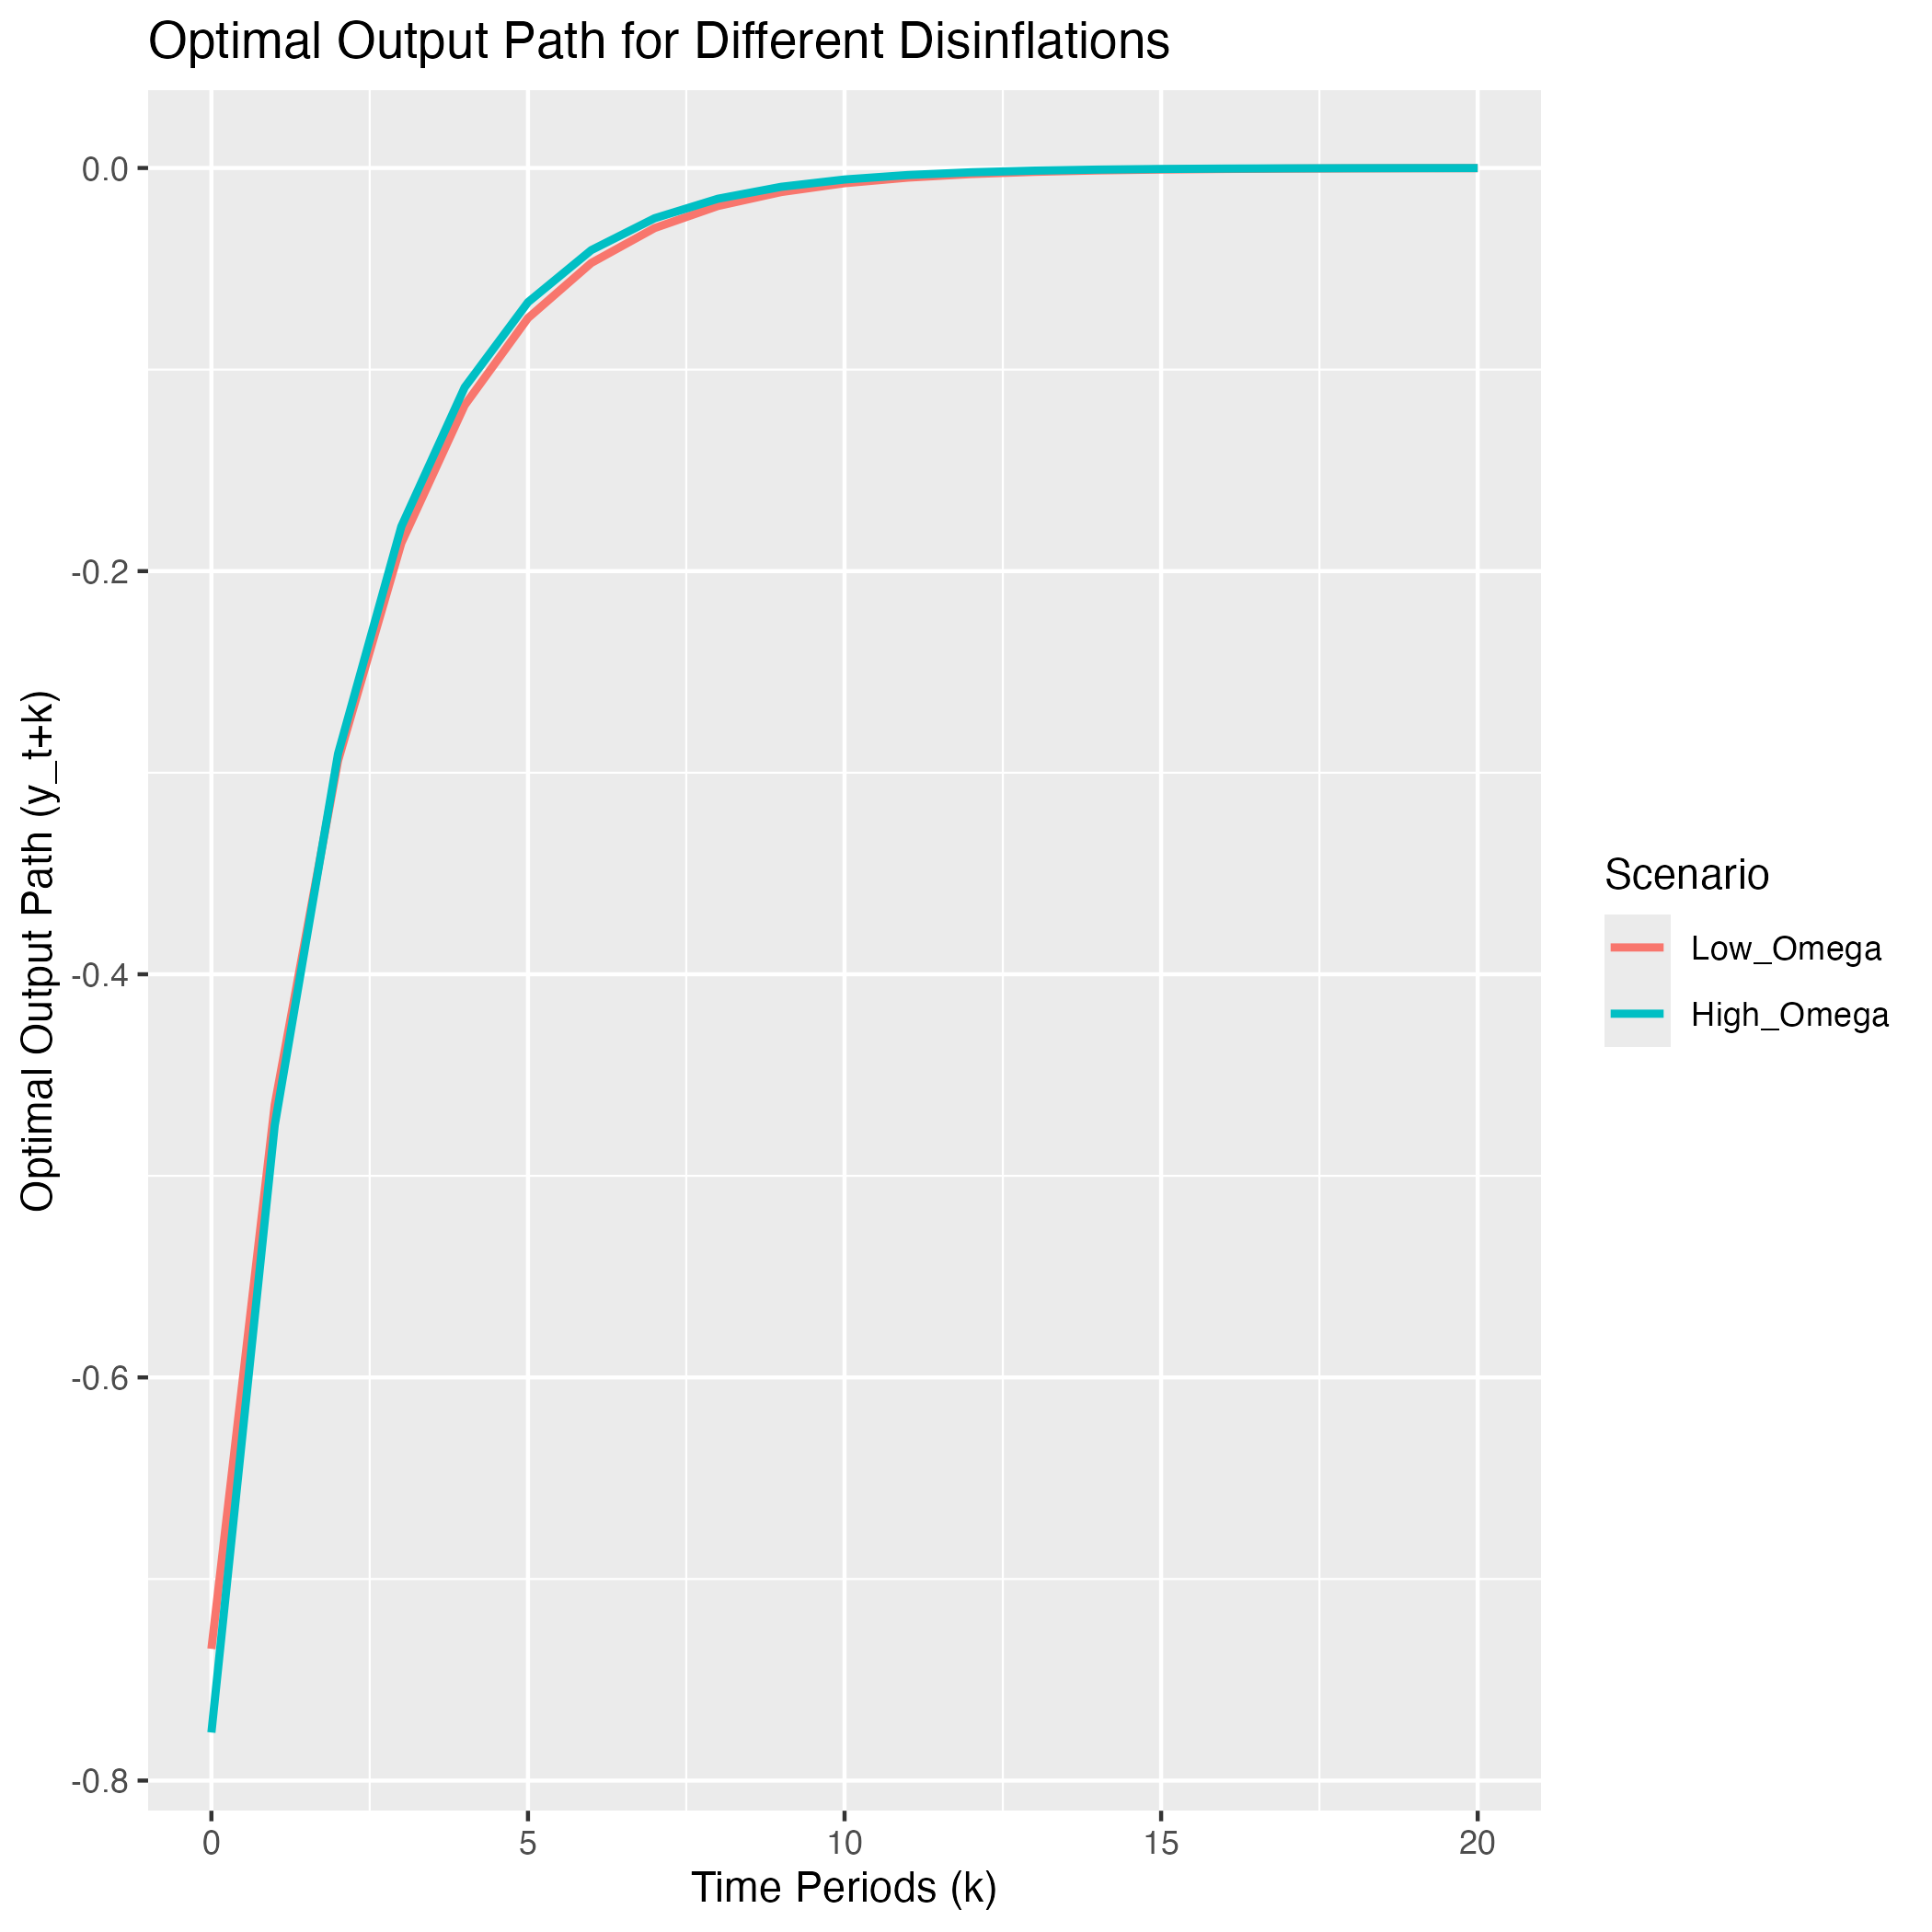
\includegraphics[width=0.8\textwidth]{/Users/cancel/Personal/Coursework/Econ425/HW8/R/optimal_output_path.png}
    \caption{Optimal Output Path for Different Disinflations}
\label{fig:optimal_output_path}
\end{figure}

\begin{figure}[ht!]
    \centering
    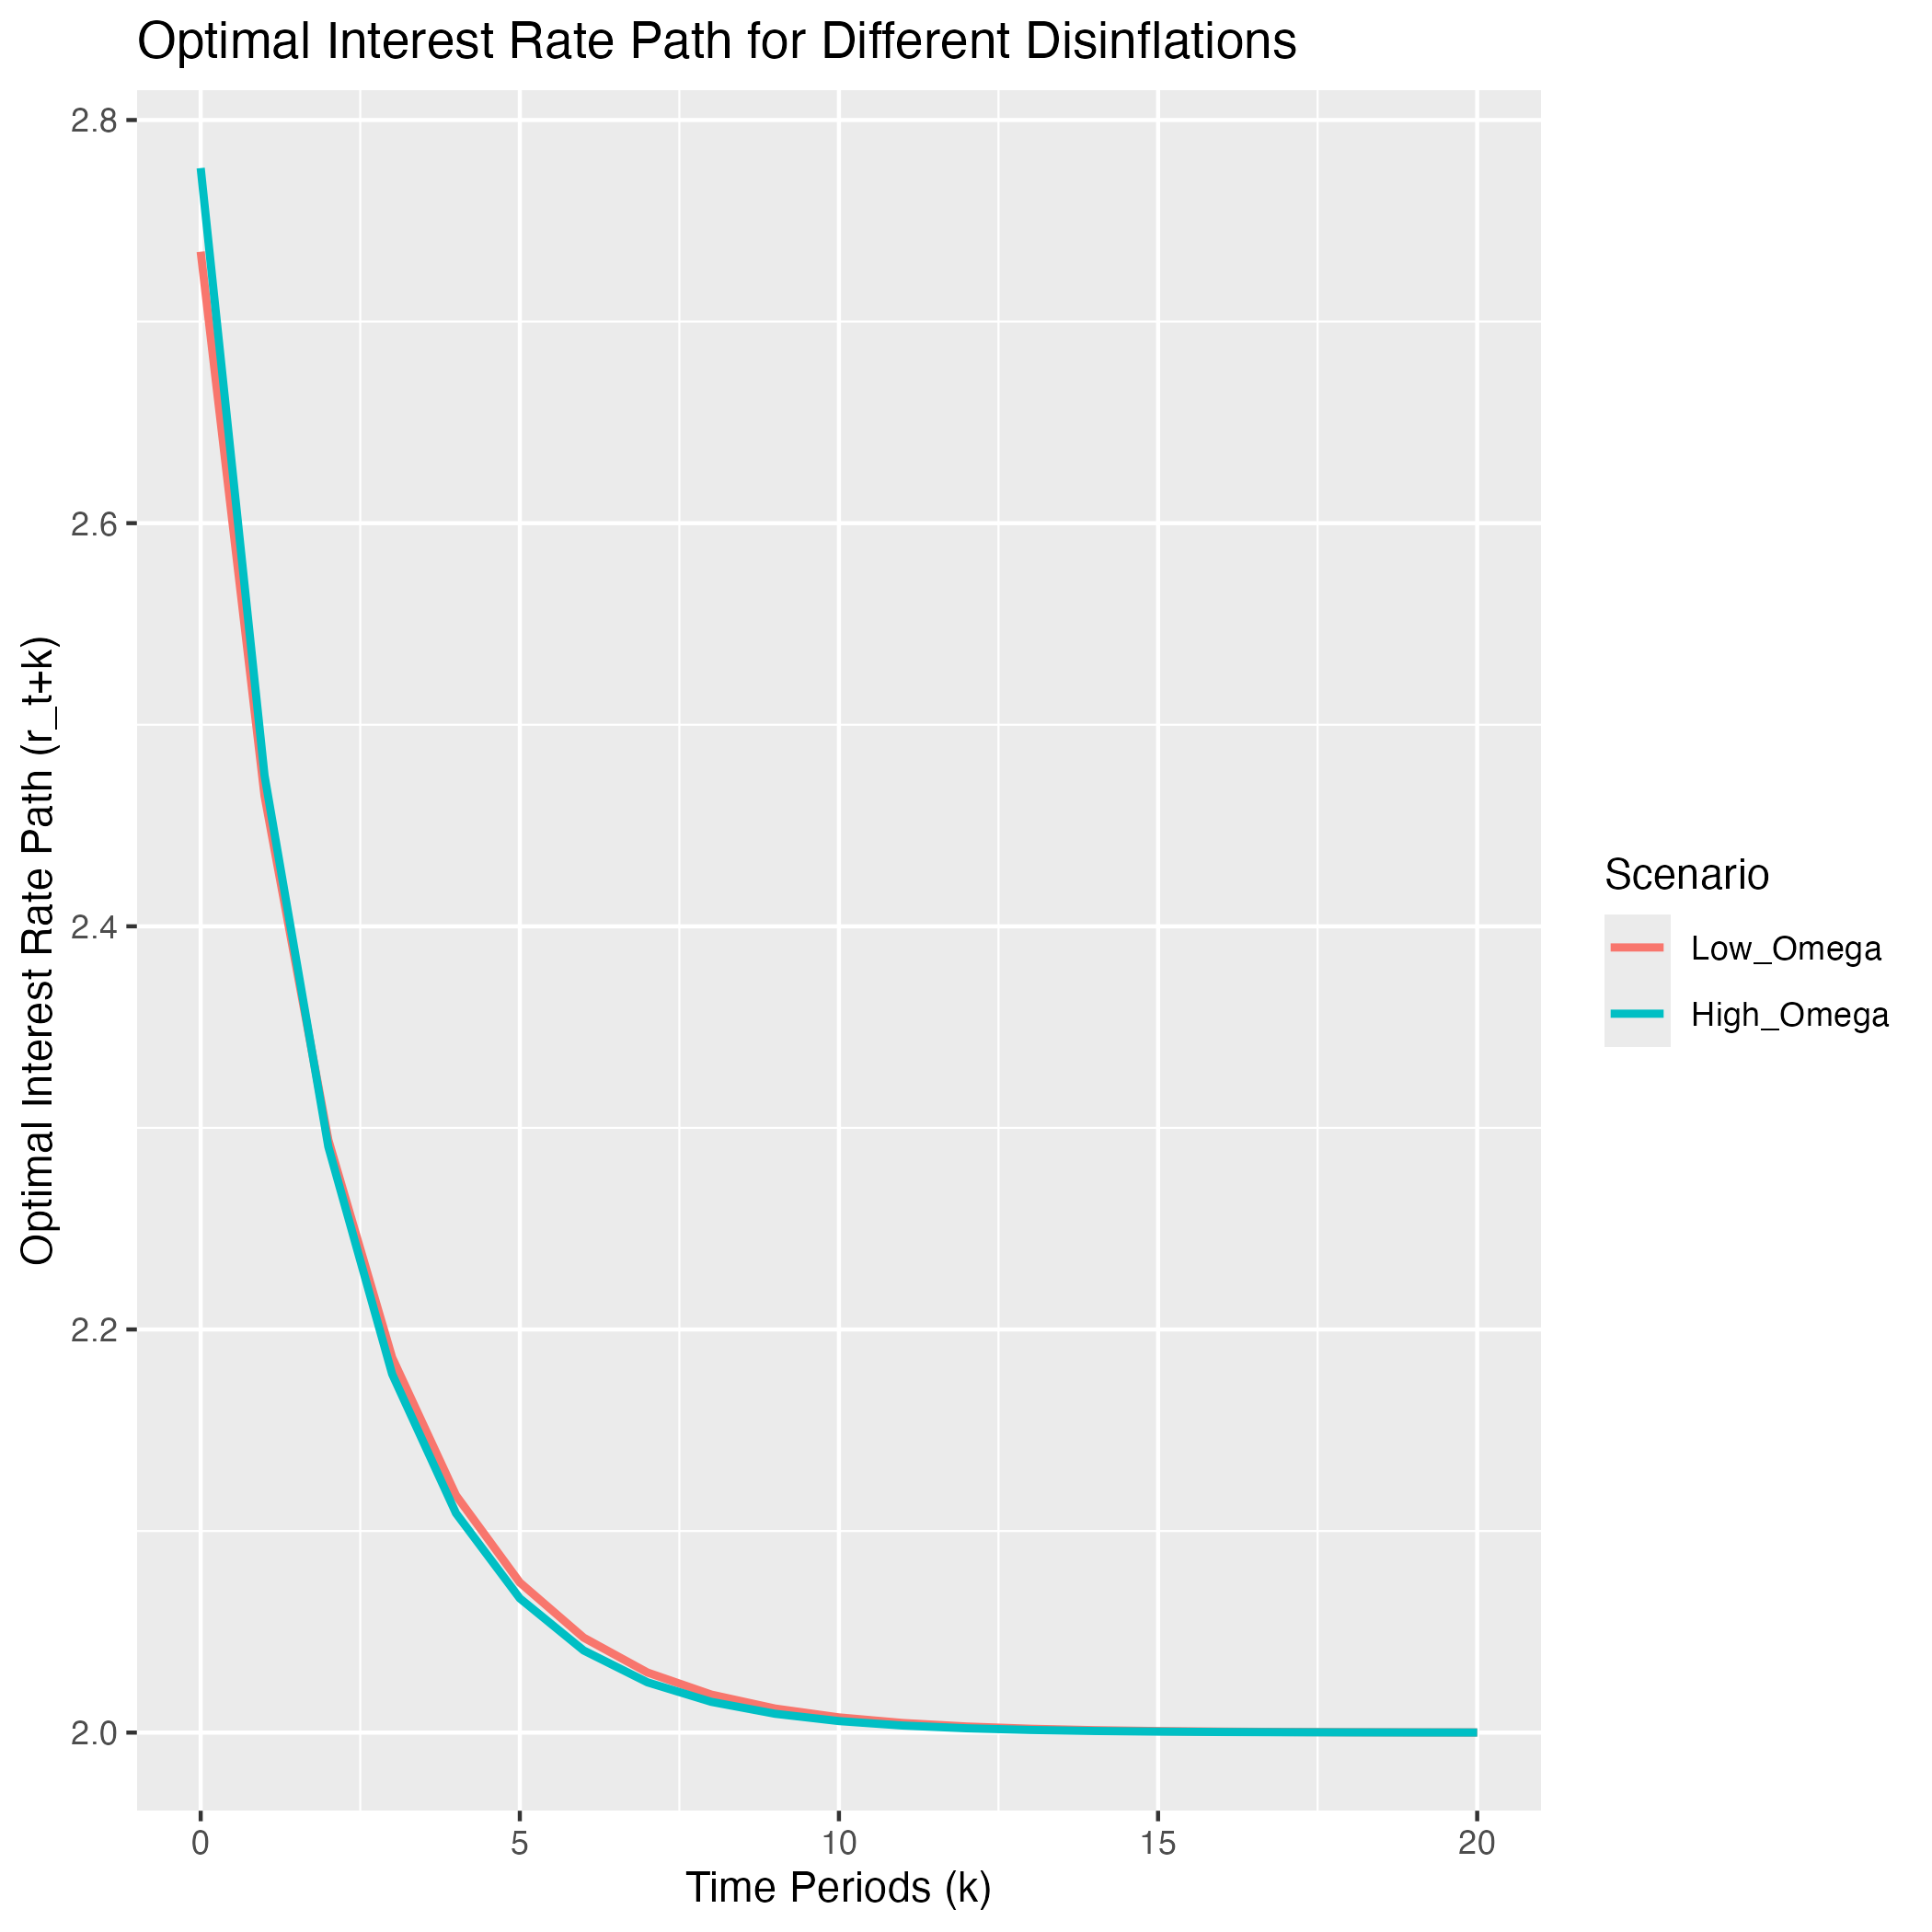
\includegraphics[width=0.8\textwidth]{/Users/cancel/Personal/Coursework/Econ425/HW8/R/optimal_interest_rate_path.png}
    \caption{Optimal Interest Rate Path for Different Disinflations}
\label{fig:optimal_interest_rate_path}
\end{figure}

\FloatBarrier

\noindent\rule{\linewidth}{0.5pt}

\subsection{Trade-offs with Aggregate Demand and Supply Shocks}

When faced with an aggregate demand shock, an optimizing central bank does not face trade-offs between its policy objectives because both output and inflation move in the same direction. The central bank can stabilize both without sacrificing one for the other.

In contrast, an aggregate supply shock creates trade-offs because output and inflation move in opposite directions. The central bank must choose between stabilizing inflation at the cost of output or vice versa. This implies that the central bank's loss function will guide its preference in dealing with such shocks, typically reflected in its choice of \(\lambda\).

\noindent\rule{\linewidth}{1pt}

\section{The Role of Expectations}

\subsection{AS Curve Components}

The AS curve is given by:
\[ \pi_t = \pi^e_{t-1,t} + \kappa (y_t - y^n_t) \]

The previous AS curve used \(\pi_{t-1}\) instead of \(\pi^e_{t-1,t}\). The main difference is that aggregate supply is centered around past inflation expectations instead of past inflation, which is generally more accurate.

\begin{itemize}
    \item \(\pi_t\): Actual inflation.
    \item \(\pi^e_{t-1,t}\): Expected inflation from the previous period.
    \item \(\kappa\): Sensitivity of inflation to the output gap.
    \item \(y_t\): Actual output.
    \item \(y^n_t\): Natural level of output.
\end{itemize}

\noindent\rule{\linewidth}{0.5pt}

\subsection{Expectation Formation}

Expectation formation refers to how economic agents form expectations about future variables such as inflation and output. These expectations play a crucial role in determining actual economic outcomes and are a key consideration in the formulation of monetary policy.

\noindent\rule{\linewidth}{0.5pt}

\subsection{Constant Expectations}

Constant expectations are when expectations of the immediate future value of a variable are the same for any time period. In other words, people always expect the immediate future value of a variable to be the same constant.

\textbf{Implications:}
\begin{itemize}
    \item No correction of expectational errors at all (even if the deviation was significant from reality).
    \item Implies the central bank can tolerate high inflation to get persistent low employment (impossible).
\end{itemize}

\noindent\rule{\linewidth}{0.5pt}

\subsection{Static Expectations}

Static expectations mean that agents use the last observed value to predict future values.

\textbf{Comparison with Constant Expectations:}
\begin{itemize}
    \item Static expectations imply that the expected value of \(x_{t+1}\) is \(x_t\).
    \item Both constant and static expectations assume no change from the last observed value.
    \item Both can be inaccurate in the face of changing economic conditions.
\end{itemize}

\textbf{Implications:}
\begin{itemize}
    \item If a central bank tries to keep the output gap at a positive, constant level, it could lead to increasing inflation over time.
    \item This situation relates to the original Phillips Curve, suggesting a trade-off between inflation and unemployment, but with static expectations, this trade-off might not hold in the long run.
\end{itemize}

\noindent\rule{\linewidth}{0.5pt}

\subsection{Rational Expectations}

Rational expectations are formed when agents use all available information and economic models to predict future variables.

\textbf{Implications:}
\begin{itemize}
    \item With rational expectations, agents anticipate the effects of monetary policy, potentially neutralizing some of its impact.
    \item Rational expectations ensure that there is no systematic error in expectation, meaning only "truly" unexpected events can cause deviations. This leads to more effective policy.
\end{itemize}

\noindent\rule{\linewidth}{0.5pt}

\subsection{Expectation Biases}

\textbf{Under Rational Expectations:}
\begin{itemize}
    \item Biases are minimized because agents use all available information.
    \item The output gap is more stable as agents adjust their behavior based on anticipated policies.
\end{itemize}

\textbf{Under Constant Expectations:}
\begin{itemize}
    \item Biases can be significant due to unanticipated changes in economic conditions.
    \item Expectations do not lag behind reality; they never account for reality. Thus, the bias could be massive and would not be resolved.
    \item The output gap might be more volatile as agents' expectations do not adjust to actual conditions.
\end{itemize}

\noindent\rule{\linewidth}{0.5pt}

\subsection{The Lucas Critique}

The Lucas Critique states that economic policies cannot be evaluated based solely on historical data because agents change their behavior in response to policies.

\textbf{Implications for Policy Evaluation:}
\begin{itemize}
    \item Policies must account for changes in agents' expectations and behaviors.
    \item The Rational Expectations Revolution emphasized the need for policies to be credible and well-communicated to be effective.
    \item The Lucas Critique suggests that trying to take advantage of certain trends or historical relationships between variables to manipulate the economy in a positive direction may not work as expected, particularly if there is no deep understanding or framework for how these variables get their value and relate.
\end{itemize}

\noindent\rule{\linewidth}{1pt}

\section{Monetary Policy as a Dynamic Game}

Assume that the policy targets are \( y > 0 \) and \( \pi = 0 \), that the Rational Expectations AS curve holds, and that \( E_{t-1} [y^n_t] = 0 \) and \( E_{t-1} [(y^n_t)^2] > 0 \) are constant.

\noindent\rule{\linewidth}{0.5pt}

\subsection{Strict Policy Rule}

Under a strict policy rule implemented by a robot, the optimal policy rule is:
\[ \pi^R_t = -\frac{\kappa}{1 + \kappa^2 / \lambda} y^n_t \]
and the corresponding level of output:
\[ y^R_t = \frac{1}{1 + \lambda / \kappa^2} y^n_t \]

\textbf{Interpretation:}
\begin{itemize}
    \item \(\lambda\) and \(\kappa\) are constant values.
    \item The expected value of \( y_t^{OR} \) must be equal to the expectation of the constant values times \( y_t^n \). Since the expected value of \( y_t^n \) is 0, the expected value of \( y_t^{OR} \) is 0. However, we were hoping to achieve a target of \( \bar{y} > 0 \), which is not the case.
    \item By the same logic (using \(\pi_t^{OR}\) instead of \(y_t^{OR}\)), we have that the expected value of \(\pi_t^{OR}\) is 0, which aligns with our target of \(\pi = 0\).
\end{itemize}

\noindent\rule{\linewidth}{0.5pt}

\subsection{Monetary Policy as a Dynamic Game}

In reality, monetary policy is not implemented by robots. It is better to think of monetary policy as a dynamic game between the central bank and the public.

\textbf{Game Structure:}
\begin{itemize}
    \item In the first period (t-1), the public forms inflation expectations.
    \item In the second period (t), the central bank sets monetary policy, taking the public's expectations as given.
\end{itemize}

\noindent\rule{\linewidth}{0.5pt}

\subsection{Equilibrium Outcomes with Discretion}

With discretion, the game leads to the following levels of inflation and output:
\[ \pi^D_t = \frac{\lambda \bar{y}}{\kappa} - \frac{\kappa}{1 + \kappa^2 / \lambda} y^n_t \]
\[ y^D_t = \frac{1}{1 + \lambda / \kappa^2} y^n_t \]

\textbf{Interpretation:}
\begin{itemize}
    \item The expected value of \(\pi_t^D\) is now greater than 0 while the expected value of \(y_t^D\) is still 0. This result is called inflation bias and is a natural result of people expecting the central bank to attempt to keep output above its natural level.
    \item This way of thinking suggests that an independent central bank is more effective. By removing the temptation to attempt to unnaturally boost economic output, people will trust the central bank to act in everyone's best interest, and as a result, inflation bias is lowered.
\end{itemize}

\textbf{Comparison with Optimal Rule:}
\begin{itemize}
    \item The discretionary policy results in an inflation bias because the central bank cannot commit to future policies.
    \item The bias arises from the central bank's incentive to exploit the short-term trade-off between inflation and output.
    \item This framework helped motivate the move towards independent central banks to reduce the inflation bias and enhance policy credibility.
\end{itemize}

\FloatBarrier

\noindent\rule{\linewidth}{1pt}
\section*{References}
\begin{enumerate}
    \item Romer, D. (2018).\ \textit{Advanced Macroeconomics}. McGraw-Hill Education.
    \item Challe, E. (2019).\ \textit{Macroeconomic Fluctuations and Policies}. MIT Press.
\end{enumerate}
\end{document}